\subsection{Цель работы}
Исследование $\sigma-\pi$ разделения МО, нахождение n-орбиталей, $\pi$-электронных зарядов на атомах, содержащих $\pi$–электроны; исследование локализации $\pi$–электронов.

\begin{figure}[H]
\centering
\captionsetup{justification=centering}
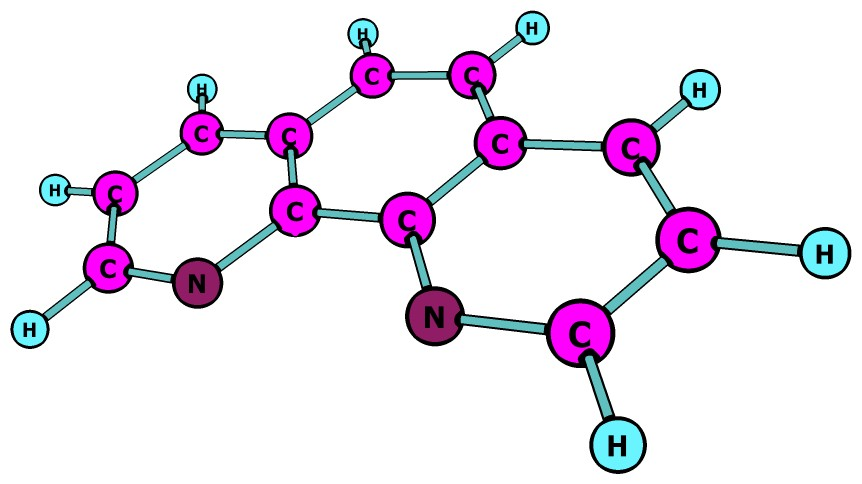
\includegraphics[scale=0.5]{fig/0.jpg}
\caption{Молекула орто-фенантролина.}
\end{figure}


\subsection{Постановка задачи}
Предварительно оптимизировать молекулярную структуру с помощью программы Avogadro, затем провести расчеты в одной точке с помощью программы GAMESS методом DFT (B3LYP) в базисе STO-3G. Проанализировать следующие показатели: 
\begin{itemize}
    \item число заполенных МО, заполненных и вакантных $\pi$-орбиталей в заданном базисе;
    \item имеет ли место у каких-либо из заполненных $\pi$-орбиталей существенная локализация на каком-то определенном атоме;
    \item имеются ли какие-либо $\sigma$-орбитали, которые можно было бы классифицировать как $n$-орбитали\footnote{Здесь и в дальнейших работах мы считаем n-орбиталями такие заполненные $\sigma$-орбитали, которые одновременно удовлетворяют следующим условиям:
\begin{enumerate}
    \item располагаются энергетически либо  выше всех заполненных $\pi$-орбиталей, либо среди высших из них; 
    \item локализованы преимущественно на тех атомах, на которых химические соображения предполагают наличие неподеленных пар электронов (одной или нескольких).
\end{enumerate}{}};
    \item по матрице плотности определить $\pi$-электронные заряды на атомах.
\end{itemize}


\subsection{Теоретическая информация}
\subsubsection{Разделение $\pi$- и $\sigma$-электроннов.}
Для плоских молекул МО можно разбить на две группы: орбитали, симметричные относительно отражения в плоскости молекулы ($\sigma$-орбитали), и орбитали, антисимметричные относительно такого отражения ($\pi$-орбитали). $\sigma$-электроны имеют максимальную вероятность нахождения в плоскости молекулы и поэтому локализованы близ нее, $\pi$-электроны – наоборот. $\pi$-электроны слабее связаны с остовом молекулы, более подвижны, легче ионизируются и более активны во взаимодействиях. Поэтому свойства ненасыщенных и ароматических систем – высокая реакционная способность, зависимость от донорных и акцепторных заместителей, спектры и т.д. – определяются, в основном, именно $\pi$-электронами.

\begin{figure}[H]
\centering
\captionsetup{justification=centering}
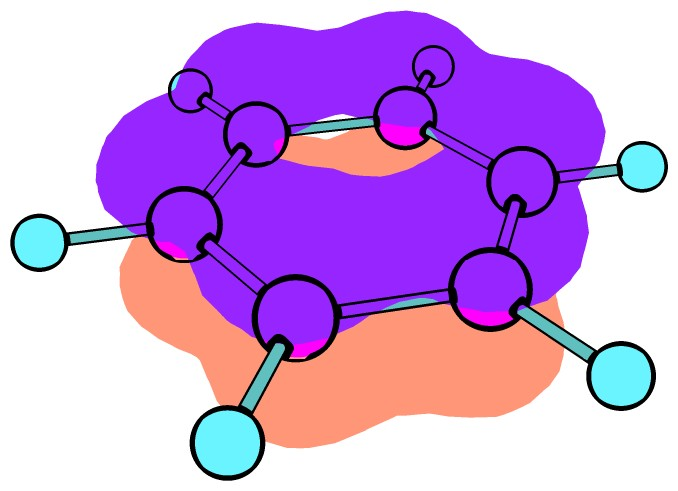
\includegraphics[scale=0.4]{fig/2.jpg}
\caption{$\pi$-орбиталь в молекуле бензола.}
\end{figure}

\begin{figure}[H]
\centering
\captionsetup{justification=centering}
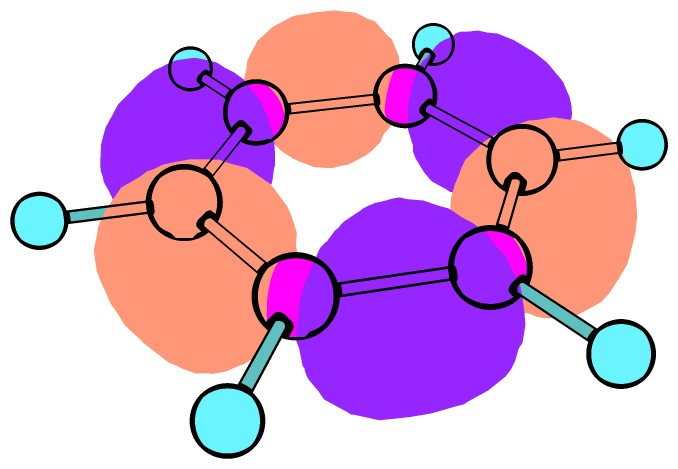
\includegraphics[scale=0.4]{fig/3.jpg}
\caption{$\sigma$-орбиталь в молекуле бензола.}
\end{figure}


\subsection{Результаты}
\paragraph*{Анализ молекулярных орбиталей}
Число МО 78, из них заполнено 47. Число заполненных $\pi$-орбиталей 7 (33, 38, 41-45). Число вакантных $\pi$-орбиталей 7 (48-54) (разделы NUMBER OF OCCUPIED ORBITALS, EIGENVECTORS).
\paragraph*{Анализ заполненных $\pi$-орбиталей}
Среди заполненных $\pi$-орбиталей у 45-ой имеется существенная локализация на атомах C5 и C6. Соответствующие коэффициенты вкладов $p_z$-орбиталей: 0.407891 и 0.407891 (раздел EIGENVECTORS). Вероятно это связано с тем, что они наиболее удалены от атомов азота (см. \ref{img:img4}).
\paragraph*{Анализ n-орбиталей}
Имеется 2 $\sigma$-орбитали, которые можно классифицировать как n-орбитали. Информация о них приведена ниже (раздел EIGENVECTORS):

\begin{table}[H]
\caption{n-орбитали в молекуле орто-фенантролина} \label{tab:tab1}
\begin{center}
    \begin{tabular}{|c|c|}
    \hline
    Номер n-орбитали & \begin{tabular}[c]{@{}c@{}}Атомы, на которых имеется\\ преимущественная локализация\end{tabular} \\ \hline
    46 & N1, N2 \\ \hline
    47 & N1, N2 \\ \hline
    \end{tabular}
\end{center}
\end{table}

Они действительно удовлетворяют критериям, по которым мы классифицируем $\sigma$-орбитали как n-орбитали: они находятся энергетически выше всех заполненных $\pi$-орбиталей, атомы азота имеют одну неподеленную электронную пару на 2s-подуровне.

\paragraph*{Анализ вкладов $\pi$-электронов в заряд на атомах}
$\pi$-электронные заряды на всех атомах, содержащих $\pi$-электроны, приведены в таблице ниже (раздел DENSITY MATRIX):

\begin{table}[H]
\caption{$\pi$-электронные заряды на атомах}\label{tab:tab2}
\begin{center}
    \begin{tabular}{|c|c|}
    \hline
    Атом & $\pi$-электронный заряд, $e$ \\ \hline
    N1 & 0.85 \\ \hline
    N2 & 0.85 \\ \hline
    C1 & 0.79 \\ \hline
    C2 & 0.79 \\ \hline
    C3 & 0.76 \\ \hline
    C4 & 0.76 \\ \hline
    C5 & 0.79 \\ \hline
    C6 & 0.79 \\ \hline
    C7 & 0.78 \\ \hline
    C8 & 0.78 \\ \hline
    C9 & 0.78 \\ \hline
    C10 & 0.78 \\ \hline
    C11 & 0.79 \\ \hline
    C12 & 0.79 \\ \hline
    \end{tabular}
\end{center}
\end{table}

\begin{figure}[H]
\centering
\captionsetup{justification=centering}
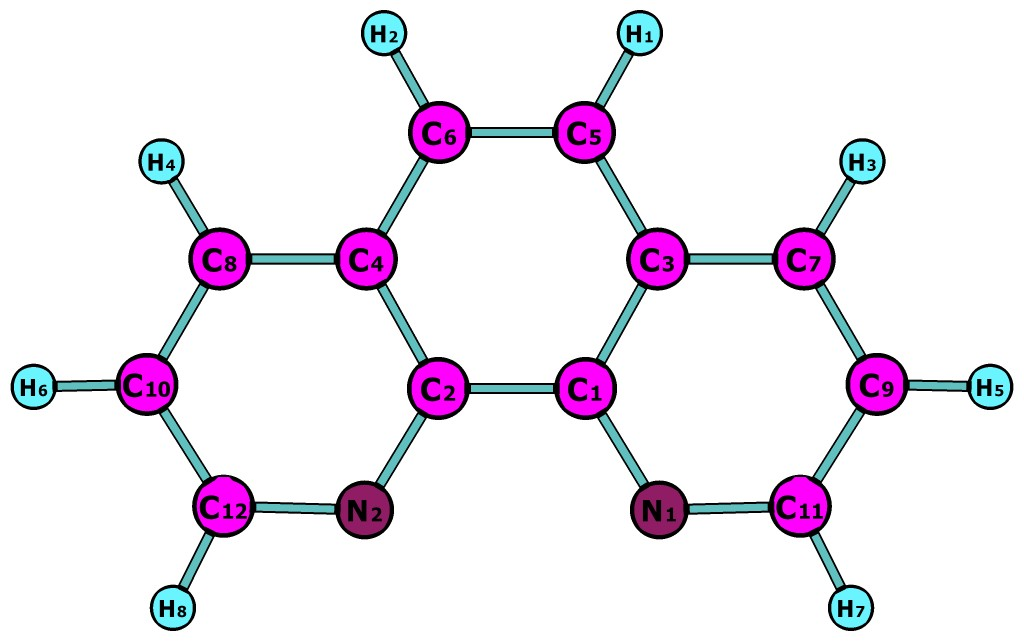
\includegraphics[scale=0.4]{fig/1.jpg}
\caption{Молекула орто-фенантролина.}
\label{img:img4}
\end{figure}


\subsection{Выводы}
\begin{enumerate}
    \item Молекула обладает симметрией, что проявляется в симметричном распределении $\pi$-электронных зарядов на атомах;
    \item на атомах азота содержится больше $\pi$-электронных зарядов, чем на атомах углерода, так как азот более электроотрицателен.
\end{enumerate}{}

\subsection{Контроль результатов}
\begin{enumerate}
    \item МО разделяются на 2 группы: у одних все коэффициенты МО при $p_z$-AO равны нулю ($\sigma$-орбитали), а у других только коэффициенты при $p_z$-AO не равны нулю;
    \item число n-орбиталей соответствует числу неподеленных пар: два атома азота, у каждого по одной неподеленной паре.
\end{enumerate}

\subsection{Приложенные файлы}
\begin{itemize}
    \item Phenanthroline.cml – исходный файл в формате cml;
    \item Phenanthroline.inp – исходные данные GAMESS для расчета методом DFT (B3LYP) в базисе STO-3G;
    \item Phenanthroline.log – результат расчета методом DFT (B3LYP)  в базисе STO-3G.
\end{itemize}{}